%!TEX root = ../thesis.tex
%Adding the above line, with the name of your base .tex file (in this case "thesis.tex") will allow you to compile the whole thesis even when working inside one of the chapter tex files

\chapter{Targets, Instrumentation, and Observations}
\label{chap:3}

Two unique data sets were analyzed as part of this thesis. The first data set was a millimeter interferometric multi-configuration study of Betelgeuse's circumstellar envelope at 1.3 mm. In the first half of this chapter we give a detailed introduction to Betelgeuse and discuss our current understanding of the star and its complex stellar atmosphere. We give a description of the millimeter interferometer CARMA, which we used to study its complex outflow region on a number of spatial scales and also describe our observations which spanned $\sim 2.5$ yr. The second data set consisted of a multi-wavelength centimeter study of two non-dusty red gaints, Arcturus and Aldebaran. In the second half of this chapter we give a detailed introduction to both of these stars, including a description of their stellar properties, and their existing atmospheric models which we test against our data in Chapter \ref{chap:6}. We give a short discription of the VLA, which was the centimeter interferometer we used to study these stars, and finally describe our VLA observations.

\section{Betelgeuse}\label{sec:3.1}
Betelgeuse ($\alpha$ Ori: M2 Iab) is the second closet red supergiant [D = 197 pc \citep{harper_2008}, barely losing that honor to Antares ($\alpha$ Sco: M1.5 Iab + B2.5 V)], and subtends the largest angular diameter of any star in the northern sky apart from the Sun. It is by far the best studied red supergiant and has been observed with various techniques from the radio to the UV. According to \cite{harper_2001}, Betelgeuse probably was a runaway star from the star-formation region Ori OB1 \cite[see, e.g.,][]{hoogerwerf_2000}, and was a spectral type O9 V star while on the main sequence where it had a mass of $\sim 20 \ M_{\odot}$. The evolutionary models of \cite{meynet_2003} suggest that its current mass is $18 \ M_{\odot}$ which corresponds to a surface gravity of 0.5 cm s$^{-2}$  (i.e., $2\times 10^{-5}g_{\odot}$). Its mass loss is characterized by a low velocity wind ($10-17$ km s$^{-1}$) and a mass loss rate of $\sim 2\times 10^{-6} \ M_{\odot} \ \rm{yr}^{-1}$ \citep{harper_2001}. Like most late-type evolved stars, Betelgeuse's  terminal wind velocity $v_{\infty}$ is smaller than the surface escape speed $v_{\rm{esc}}$ (values given in Table \ref{tab:3.1}). This means that most of the energy and momentum are deposited into its flow within the first few stellar radii.

\begin{table}[!hbt]
\begin{center}
\caption[Physical Properties of $\alpha$ Ori.]
{Physical Properties of $\alpha$ Ori.}
\begin{tabular}{lcc}
\hline
\hline
\rule{0pt}{2.5ex}Property & Value & Reference \\
\hline
\rule{0pt}{2.5ex}HD Number & 39801 & $\ldots$\\
Spectral Type & M2 Iab & \cite{perryman_1997} \\ 
App. Mag. (V) & 0.45 & \cite{perryman_1997}\\
RA (ICRS: ep=J2000)& 05$^{\rm{h}}$55$^{\rm{m}}$10.305$^{\rm{s}}$ & \cite{van_leeuwen_2007}\\
dec (ICRS: ep=J2000) & +07$^{\circ}$24$^{\prime}$25.430$\arcsec$& \cite{van_leeuwen_2007}\\
Proper motion-RA (mas yr$^{-1}$)& 27.54 & \cite{van_leeuwen_2007}\\
Proper motion-dec (mas yr$^{-1}$)& 11.30 & \cite{van_leeuwen_2007}\\
$\pi$ (mas)& $5.07\pm1.1$ &\cite{harper_2008}\\
d (pc)& $197\pm45$ & \cite{harper_2008}\\
Main Sequence $M_{\star}$ ($M_{\odot}$) & $\sim 20$ & \cite{meynet_2003}\\
Main Sequence Spectral Type & O9 V & \cite{harper_2008}\\
Current $M_{\star}$ ($M_{\odot}$) & $\sim 18$ & \cite{meynet_2003}\\
$\theta _{\rm{UD}}$ (mas)& $43.33 \pm 0.04$ & \cite{perrin_2004}\\
$R_{\star}$ ($R_{\odot}$)& 950 & \cite{harper_2008} \\
$T_{\rm{eff}}$ (K)& 3650 & \cite{levesque_2005}\\
Log $L_{\star}/L_{\odot}$& $5.10\pm0.22$  & \cite{harper_2008}\\
$g_{\star}$ (cm s$^{-2}$ )& 0.5 & \cite{meynet_2003} \\
Heliocentric $v_{\rm{rad}}$ (km s$^{-1}$) & $20.7\pm0.4 $& \cite{harper_2008} \\
$v_{\rm{esc}}$ (km s$^{-1}$) & 85 & \dots\\
$v_{\rm{\infty}}$ (km s$^{-1}$)& 10, 17 & \cite{bernat_1979} \\
$T_{\rm{wind}}$ (K)& $< 4000$ & \cite{lim_1998} \\
$\dot{M}_{\star}$ ($M_{\odot}$ yr$^{-1}$)& $3\times 10^{-6}$ &\cite{harper_2001} \\
Photospheric $H_{\star}$ ($R_{\star}$)& 0.006 & $\dots$\\
Fe/H& $0.05 \pm 0.14$ & \cite{ramirez_2000}\\
O/C& 2.5 & \cite{lambert_1984}\\
Rotational period (yr) & 17 & \cite{uitenbroek_1998}\\
$B_{\star}$ (G) & $\sim 1$ & \cite{auriere_2010} \\
Chromosphere Model & $\ldots$ & \cite{harper_2001} \\
Wind Model &  $\ldots$ &\cite{harper_2001}\\ 
Outer CSE &  $\ldots$ &\cite{rodgers_1991}\\ 
$^{12}$C/$^{13}$C & $6\pm 1$ &\cite{harris_1984}\\ 
$^{16}$O/$^{17}$O & $525\pm 250$ &\cite{harris_1984}\\ 
$^{16}$O/$^{18}$O & $700\pm 300$ &\cite{harris_1984}\\ 
\hline
\rule{0pt}{2.0ex}
\end{tabular}
\label{tab:3.1}
\end{center}
\end{table}

Betelgeuse has an extremely slow rotation period of about 17 yr \citep{uitenbroek_1998} which implies that it is probably experiencing very limited action of a solar-like dynamo. Its large radius ($950 \ R_{\odot}$) means that any possible remanent of a strong main sequence magnetic field is likely negligible due to a large dilution factor. In comparison to Sun like stars, its large radius also means that it has a large photospheric scale height ($H_{\star} \sim 0.01 \ R_{\star}$). The expected result of this is the presence of no more than a few giant and stable convection cells in the photosphere \cite{schwarzschild_1975}. Such features should enhance the detectability of the magnetic fields generated through a turbulent dynamo \citep{vogler_2007}. \cite{bedecarrax_2013} have recently monitored Betelgeuse over a three year period using high resolution spectropolarimetry, and find a longitudinal magnetic field strength which varies  in values ranging from $-3$ G to $+2$ G with temporal changes in the field strength occurring over timescales as short as a few weeks.

Various studies have assumed that Betelgeuse has a warm ($T_e \sim 8000$ K) extended atmosphere where ionized hydrogen dominates the electron density \citep[e.g.,][]{newell_1982,hartmann_1984}. In fact, high resolution UV imaging with the HST partially resolved the \textit{hot} chromosphere revealing $6000-8000$ K plasma extending to more than 2 $R_{\star}$ \citep{gilliland_1996}. However, \cite{lim_1998} spatially resolved Betelgeuse with the `old' VLA at 5 different wavelengths and showed that the mean electron temperature is actually much cooler, i.e., $T_e = 2000 - 4000$ K and extends out to several stellar radii as shown in Figure \ref{fig3.1}. In fact, the mid-IR [\ion{Fe}{ii}] line studies of \cite{harper_2009} suggest that the temperature of the bulk of the plasma where the chromosphere has its largest filling factor is $< 2500$ K. Therefore, it appears that the hot chromospheric plasma has a small filling factor and co-exists with the much more abundant cool plasma within several stellar radii. \cite{harper_2001} constructed a detailed physical model for the inner atmosphere of Betelgeuse which reproduces the radio fluxes of \cite{lim_1998} and consists of electron temperature and gas densities as a function of radius.

\begin{figure}[hbt!]
\centering 
\mbox{
          \includegraphics[trim=0pt 0pt 0pt 0pt,clip,scale=0.33]{/home/eamon/thesis/thesis_template/3/lim1.ps}
          \includegraphics[trim=0pt 20pt 0pt 0pt,clip,scale=0.35]{/home/eamon/thesis/thesis_template/3/lim2.ps}
          }
\caption[VLA spatially resolved analysis of Betelgeuse.]{Left: The spatially resolved Q-band VLA image of Betelgeuse showing asymmetry in its atmosphere. Right: The multi-frequency spatially resolved radio maps revealed that the mean electron temperature profile was lower than expected \citep{lim_1998}.}
\label{fig3.1}
\end{figure}

In comparison to other well studied red supergiants such as VY CMa, Betelgeuse has a modest mass loss rate, a low gas-to-dust mass ratio of $200-1700$, and low molecular abundances \citep{harper_2001}. However, it is known to possess a molecular shell known as a MOLsphere above its photosphere \citep{tsuji_2000}, and recently \cite{verhoelst_2006} and \cite{perrin_2007} have used the VLTI to establish some of its properties. They find the MOLsphere to have a geometrical thin extent ($\sim 0.1 \ R_{\star}$) with a temperature of $\sim 1500$ K at $\sim 1.4 \ R_{\star}$, and contains molecules such as H$_{2}$O, SiO, and Al$_{2}$O$_{3}$. Notably, they suggest that this molecular layer is where dust nucleation commences in support of a dust-driven wind scenario. However, the existence of Al$_{2}$O$_{3}$ is disputed by \cite{kaminski_2013} who argue that the absence of AlO (which is required to form Al$_{2}$O$_{3}$) in the photospheric spectrum is puzzling, and verification by independent studies is needed. In addition, \cite{woitke_2006} finds that the average temperature between $1-3 \ R_{\star}$ is too high for silicates to form, and indeed recent studies suggest that silicates are not formed inside $\sim 23 \ R_{\star}$ \citep{skinner_1997,tatebe_2007}. For Betelgeuse, it therefore appears that radiation pressure on dust grains is not the main mechanism driving its mass loss \citep{harper_2010}.

In the past decade or so, a number of sensitive multi-wavelength studies of Betelgeuse have revealed a complex non-spherically symmetric circumstellar environment. Starting at its surface, a $H$ band interferometric image was reconstructed using data from the Infrared Optical Telescope Array (IOTA) and showed a non-uniform brightness distribution across its surface \citep{haubois_2009}. This data was modelled with 3-D hydrodynamical simulations by \cite{chiavassa_2010}, resulting in the detection of a granulation pattern on the surface. They concluded that  the surface contains a large ($\sim 30$ mas) convective cell and a few small to medium scale ($5-15$ mas) convection-related surface structures. Adaptive optics images with the Very Large Telescope (VLT) at $1.04 -2.17 \ \mu m$ revealed an irregular circumstellar envelope at a few $R_{\star}$ with a few bright plumes extending out to 6 $R_{\star}$ \citep{kervella_2009}. These plumes have been attributed to the action of giant convection cells. Thermal infrared VLT ($\lambda=8-20 \ \mu m$) imaging revealed oxygen-rich dust out to $100 \ R_{\star}$ ($2.5\arcsec$) \citep{kervella_2011}, while Herschel images show a chaotic dust distribution far out in the circumstellar envelope, i.e., beyond $600 \ R_{\star}$ (i.e. $> 15\arcsec$) \citep{decin_2012}. A conclusion that can be drawn from these studies is the constant presence of inhomogenities in the circumstellar environment which probably play a role in the formation of dust and molecular species. We defer a discussion on previous observations of CO in Betelgeuse's circumstellar environment until Chapter \ref{chap:5}.

\section{CARMA}\label{sec:3.2}

The Combined Array for Research in Millimeter-wave Astronomy (CARMA) \citep{bock_2006} is a millimeter interferometer located at Cedar Flat in eastern California at an elevation of 2200\,m. The array consists of nine 6.1\,m antennas and six 10.4\,m antennas formerly from the Berkeley Illinois Maryland Association (BIMA) and the Owens Valley Radio Observatory (OVRO) arrays respectively, and operates at 85-115 GHz (3 mm) and 215-270 GHz (1.3 mm). Eight additional 3.5 m antennas known as the Sunyaev-Zel'dovich Array (SZA) can also be added to CARMA for continuum observations at 26-36 GHz (1 cm) and 85-115 GHz (3 mm). The different sizes of the CARMA antennas makes it a heterogeneous array with a  total collecting area equivalent to a single 32 m dish antenna. Despite some technical difficulties associated with image restoration for a heterogeneous array (e.g., the 15-element CARMA array has 3 different primary beams), there are a number of advantages. Such an array samples shorter $u-v$ spacings directly when the smallest antennas are in a compact configuration. This results in more of the total flux density being recovered and also recovers more of the large scale structure and is the reason why the smaller diameter antennas are usually left in the center of the array as shown in Figure \ref{fig3.2}. In fact, it has been shown that a heterogeneous CARMA array produces better image fidelity than a homogeneous array with the same number of antennas and collecting area \citep{wright_1999}. 

\begin{figure}[!ht]
\centering 
          \includegraphics[trim=100pt 0pt 120pt 0pt,clip,width=\textwidth,angle=90,scale=0.42]{/home/eamon/thesis/thesis_template/3/carma_configs.ps}
\caption[The three CARMA array configurations used.]{The three CARMA array configurations used to study to CSE of Betelgeuse. The most compact CARMA configuration is E configuration (\textit{left}) which has $B_{\rm{max}}=66$ m, D configuration (\textit{middle}) has $B_{\rm{max}}=148$ m, while C configuration (\textit{right}) has $B_{\rm{min}}=370$ m and was the most extended configuration used in our study. The 10.4 m antennas are marked green while the 6.1 m antennas are marked black.}
\label{fig3.2}
\centering 
          \includegraphics[trim=0pt 300pt 0pt 250pt,clip,width=\textwidth,scale=0.42]{/home/eamon/thesis/thesis_template/3/carma_layout.ps}
\caption[The layout of antenna pads for CARMA.]{The layout of antenna pads for CARMA and a visual of the extent of each configuration \citep{bock_2006}.}
\label{fig3.3}
\end{figure}

CARMA is a reconfigurable array and has 5 different configurations providing baselines ranging between 8 m and 2 km; A configuration being the most extended and E configuration being the most compact. Figure \ref{fig3.3} gives an overview of how these configurations are achieved at Cedar Flat. As the resolution is set by the array configuration and frequency of observation, we list the various achievable resolutions (i.e. the HPBW of the synthesized beam) for each of CARMA's 5 configurations at 230 GHz, in Table \ref{tab:3.2}.  We also list the largest angular scale that can be imaged at 230 GHz as this is an important property of each configuration, especially when imaging extended emission (i.e., Chapter \ref{chap:5}). This limitation is unique to interferometers and means that structures on angular scales significantly larger than the fringe spacing formed by the shortest baseline are not measured. This information can only be obtained by observing in a smaller array configuration or by using the mosaicing method. The half-power beamwidth of the primary beam (i.e., the FOV) at a frequency $\nu$ is $50\arcsec \times (230\,\rm{GHz}/\nu)$ for the 6.1 m antennas, while is $30\times  \arcsec(230\,\rm{GHz}/\nu)$ for the 10.4 m antennas.

\begin{table}[!hbt]
\begin{center}
\caption[Properties of the 5 CARMA configurations.]
{Properties of the 5 CARMA configurations.}
\begin{tabular}{lccccc}
\hline
\hline
\rule{0pt}{2.5ex} & A & B & C & D & E \\
\hline
\rule{-4.0pt}{2.5ex} $B_{\rm{max}}$ (m) &1883 \ \ & 946 \ \ & 370 \ \ & 148 \ \ & 66 \ \ \\
$B_{\rm{min}}$ (m)& 150& 82& 26& 11& 8.5\\ 
Synthesized Beam $\theta _{\rm{HPBW}}$ ($\arcsec$)& 0.15& 0.38& 0.86& 2.1& 4.4\\ 
Largest Angular Scale $\theta _{\rm{LAS}}$ ($\arcsec$) & 1.1& 2.0& 6.2& 14.6& 18.9\\ 
\hline
\rule{-4.0pt}{2.5ex} 6.1 m Primary Beam $\theta _{\rm{HPBW}}$ ($\arcsec$) & \multicolumn{5}{c}{$50\times \arcsec(230\,\rm{GHz}/\nu)$} \\ 
10.4 m Primary Beam $\theta _{\rm{HPBW}}$ ($\arcsec$) & \multicolumn{5}{c}{$30\arcsec \times (230\,\rm{GHz}/\nu)$} \\ 
\hline
\rule{0pt}{2.0ex}
\end{tabular}
\label{tab:3.2}
\end{center}
\end{table}
\begin{figure}[!ht]
\centering 
          \includegraphics[trim=20pt 220pt 20pt 200pt,clip,width=\textwidth,scale=0.45]{/home/eamon/thesis/thesis_template/3/carma_path.ps}
\caption[Major components in the signal path for CARMA.]{Major components in the signal path through the CARMA system \citep{wei_2008}.}
\label{fig3.4}
\end{figure}
The 10.4 meter and 6.1 meter antennas are equipped with circular polarization  SIS receivers for the 1mm band, and single-polarization SIS receivers for the 3 mm band. The tuning ranges of the 1mm and 3mm receivers are 215-265 GHz and 85-116 GHz, respectively. Figure \ref{fig3.4} shows the main components in the signal path through the CARMA system. Upon passing through the atmosphere and antenna Naysmith optics, the RF signal is sent through the cooled low noise double sideband mixer where it is combined with a local oscillator $\nu _{\rm{LO1}}$ to produce the intermediate frequency $\nu _{\rm{IF}}$. The $\nu _{\rm{LO1}}$ can be either below or above the $\nu _{\rm{RF}}$; known as the upper and lower sidebands, respectively, giving:
\begin{equation}
\nu _{\rm{IF}}=\nu _{\rm{RF}}\pm \nu _{\rm{LO1}}.
\end{equation}
The radio frequency gain $G_{\rm{RF}}(\nu _{RF})$, results from components before this mixer (i.e., the sky and antenna optics) and depends only on the sky frequency. The IF signals then pass through amplifiers and attenuators in the antenna, are converted to light and sent along fibers to the control building, where they are then converted back to microwaves, amplified and attenuated some more before reaching the second mixer. Even though many of the components in the IF path are common across all bands, the IF gain $G_{\rm{IF}}$($\nu _{\rm{IF}}$ ), will vary per band as there are components in the second mixer which are separate for each band. The second mixer is a single sideband mixer and its baseband output contains either the upper sideband signals above the second LO or the lower sideband:
\begin{equation}
\nu _{\rm{BB}} = \nu _{\rm{IF}} \pm \nu _{\rm{LO2}}.
\end{equation}
A noise signal is passed through all of the remaining correlator configuration dependent components and the selectable analog filters are measured by this noise source. The power measurement $P_{\rm{sys}}$, used for the system noise temperature measurement is calculated after the analog filters and before the automatic level control (ALC) amplifier which ensures that the digitizers operate at a constant level.

\section{CARMA Observations of Betelgeuse}\label{sec:3.3}
We used CARMA to obtain on-source profiles of the rotational transition line $\rm{{}^{12}}$C$\rm{{}^{16}}$O($J=$ 2-1) which has a rest frequency of 230.538\,GHz (1.3\,mm). Table \ref{tab:3.3} summarizes our complete set of multi-configuration observations which span the period 2007 May - 2009 November. Our first set of observations took place in June 2007 when CARMA was in D configuration providing a spatial resolution of $2.1\arcsec$. A total of 5 D configuration tracks were carried out and one which took place in 18 May 2007 was excluded from the final analysis due to large levels of noise in the final map as a result of poor weather conditions. We obtained five E configuration (the most compact configuration available) tracks during the summer of 2009  which provided a relatively low spatial resolution of $4.4\arcsec$ but gave the best sensitivity to extended emission. However, only one track was found to be of sufficient quality to be included in the final analysis. Our C configuration observations which provide sub-arcsecond resolution at 230 GHz (i.e., $0.9\arcsec$) were due to take place in December 2008 but were postponed for a full year due to very poor weather conditions at  Cedar Flat. We obtained a total of 4 usable tracks in C configuration amounting to 8.4 hours on source. The FOV of the individual 10.4\,m antennas is $\sim$ 32$\arcsec$ at the observed frequency.

CARMA can now take measurements in eight bands yielding a maximum bandwidth of 4 GHz per sideband. However, back when our data was obtained, the CARMA correlator took measurements in just three separate bands, each having an upper and lower sideband. One band was set to the low resolution 468\,MHz bandwidth mode (15 channels of 31.25\,MHz each) to observe continuum emission and was centered on the line. The other two bands were configured with 62\,MHz and 31\,MHz bandwidth across 63 channels (with a resolution of $1.3\>{\rm km\>s}^{-1}$ and $0.65\>{\rm km\>s}^{-1}$ respectively) and were also centered on the line. The line was measured in the upper sideband in the C and E array and in the lower sideband in the D array.

Bandpass and phase calibration were performed using 3C120 and 0530+135. 0532+075 was used as a secondary phase calibrator to determine the quality of the phase transfer from the primary phase calibrator. The observing sequence was to integrate on the primary phase calibrator for $\sim$ 2.5 minutes, the target for $\sim$ 18 minutes, and the secondary phase calibrator for $\sim$ 2.5 minutes. The cycle was repeated for each track which lasted between 1.5 hours and 5 hours. Absolute flux calibration was carried out with 0530+135 and 3C120 using the continuously updated CARMA flux catalog to obtain their flux values at each observation.

%\afterpage{
\begin{landscape}
\begin{table}[hb!]
\begin{center}
\caption[CARMA Observations of $\alpha$ Ori.]
{CARMA Observations of $\alpha$ Ori between June 2007 and November 2009.}
\begin{tabular}{lccccc}
\hline
\hline
\rule{0pt}{2.5ex}Date & Configuration & Time on Source & Flux		& Phase 	& Image Cube \\
	 & 				 &  (hr)		  & Calibrator	& Calibrator& Dynamic Range \\
\hline
\rule{0pt}{2.5ex}2007 Jun 18 	& D & 0.9 & 0530+135	& 0530+135, 0532+075 	&  22.8 \\
2007 Jun 21 	& D & 3.0 & 0530+135	& 0530+135, 0532+075 	&  22.7 \\
2007 Jun 24 	& D & 2.1 & 0530+135	& 0530+135, 0532+075 	&  26.1 \\
2007 Jun 25 	& D & 2.4 & 0530+135	& 0530+135, 0532+075 	&  30.2 \\
2009 Jul 07	& E & 3.2 & 3C120 		& 3C120, 0532+075	& 30.1 \\
2009 Nov 05	& C & 1.2 & 3C120 		& 3C120, 0532+075 	& 17.3 \\
2009 Nov 09 	& C & 3.0 & 3C120 		& 3C120, 0532+075 	& 27.2 \\
2009 Nov 15	& C & 1.0 & 3C120 		& 3C120, 0532+075 	& 17.8 \\
2009 Nov 16	& C & 3.2 & 3C120 		& 3C120, 0532+075 	& 32.0  \\
All		& C & 8.4	&  $\dots$	& 	$\dots$	& 43.8 \\
All 		& D & 8.4 &  $\dots$	&  	$\dots$	& 31.9 \\
All 		& Multi-configuration & 20.0 & $\dots$& $\dots$ 	& 52.3 \\
\hline
%\tablenotetext{a}{Central frequency of selected bandpass.}
%\tablenotetext{b}{Number of available antennae remaining after flagging.}
\end{tabular}
\label{tab:3.3}
\end{center}
\end{table}
\end{landscape}
%}

\section{Arcturus and Aldebaran}\label{sec:3.4}

Currently the most detailed spatial information about the atmospheres of K and early M spectral type evolved stars is obtained from eclipsing binaries such as the $\zeta$ Aurigae and symbiotic systems (e.g., \citealt{wright_1970}; \citealt{baade_1996}; \citealt{eaton_2008}; \citealt{crowley_2008}). Even though these systems offer us the best opportunity to obtain information on the dynamics and thermodynamics at various heights in the evolved star's atmosphere, the very nature of the binary system may introduce further complexities. For example, the orbital separation is often within the wind acceleration region and one could expect flow perturbations to be present (e.g., \citealt{chapman_1981}). 
Using the old VLA, \cite{harper_2005} find a slow wind acceleration for $\zeta$ Aurigae and confirm that its velocity structure is not typical of single stars with similar spectral types, such as $\lambda$ Velorum \citep{carpenter_1999}.   In order to avoid the assumed additional complexities of a companion, we have selected two single luminosity class III red giants: Arcturus ($\alpha$ Boo: K2 III) and Aldebaren ($\alpha$ Tau: K5 III). These nearby red giants have been extensively studied at other wavelengths and their stellar parameters, which are summarized in Table \ref{tab:3.4}, are accurately known. These stars are predicted to be point sources at all frequencies between 1 and 50 GHz in all VLA configurations so our radio observations measure their total flux density, $F_{\nu}$. For example, our observations of these stars which are discussed in Section \ref{sec:3.6}, were taken in B configuration providing a maximum spatial resolution of $\sim 0.14 \arcsec$ at 45 GHz which is equivalent to $\sim 7\ R_{\star}$ for both stars. The radio emission from these stars at 45 GHz is expected to be chromospheric in origin \citep{harper_2013}, and as the spatial extent of red giant chromospheres is expected to be less than $1.5 \ R_{\star}$ \citep{berio_2011}, then we can be assured that these targets will be unresolved even at the highest VLA frequencies. Moreover, both stars have existing semi-empirical 1-D chromospheric and wind models which we can directly compare our data against.
\\
\\
\textbf{\textit{Arcturus ($\alpha$ Boo: K2 III)}}\\
Arcturus ($\alpha$ Boo: K2 III) is the nearest ($d=11.3$ pc) and brightest ($V=-0.04$ mag) noncoronal red giant and is probably the best example of a red giant whose atmosphere can be studied in detail with the VLA. It is the leader of a group of stars that share a similar $V$  space velocity (the component of stellar motion relative to the LSR in the direction of rotation),  age ($\geq10$ Gyr), and metallicity ([Fe/H] $\sim -0.5$), known as the Arcturus moving group \citep{eggen_1971}. The group has traditionally been regarded as the remains of a dissolved open cluster \citep[e.g.,][]{eggen_1971,eggen_1996} but it has also been suggested to be  the debris of a metal-poor accreted satellite some billions of years ago \citep{navarro_2004}. Recent analysis of chemical abundances are consistent with the former hypothesis but do not entirely rule out a merger one \citep{williams_2009}. Arcturus is ascending the red giant branch and being a single star, its mass is relatively poorly constrained but is similar to that of the Sun \citep[$0.8 \pm 0.2 \ M_{\odot}$ by][]{kallinger_2010}. During the last decade there has been a large dispersion in the reported values of Arcturus' effective temperature \citep[a nice graph summarizing this is presented in][]{griffin_1996} but nowadays it is generally accepted to be about 4300 K \citep{di_benedetto_1993}. A number of interferometric measurements of the limb-darkened angular diameter of the star are available in the literature with most values agreeing within their uncertainties. The weighted mean value of these values is $\theta _{\rm{LD}}= 21.06\pm0.17$ mas \citep{ramirez_2011} giving the star a radius of $25.4\pm 0.3\ R_{\odot}$.

Arcturus is an important target for high spatial and spectral resolution calibration. Thus when the Hipparcos catalog flagged Arcturus as a two component object \citep{perryman_1997} it caused quite a stir in the community. However, the uncertainties in the  Hipparcos data \citep{Soderhjelm_1998O} along with a non-detection in adaptive optics observations \citep{turner_1999} and sensitive interferometric techniques \citep{lacour_2008} suggest that Arcturus is single and can still be used as a calibrator. Nevertheless, \cite{lacour_2008} still do not rule out the possibility of a planetary companion of a few Jovian masses as suggested by its long period radial velocity variations of $\sim 233$ days \citep{hatzes_1993,brown_2007}. Variations in the order of a few days period are also seen in its radial velocity \citep{merline_1999} as well as photometry \citep{retter_2003}. The photometric amplitude oscillations can vary by up to a percent and may be the manifestation of convection such as large-scale granulation, or solar-like oscillations \citep{dziembowski_2001}. 

\begin{table}[!hb]\small
\begin{center}
\caption[Basic Properties of $\alpha$ Boo and $\alpha$ Tau.]
{Basic Properties of $\alpha$ Boo and $\alpha$ Tau.}
\begin{tabular}{lccc}
\hline
\hline
\rule{0pt}{2.5ex}Property & $\alpha$ Boo & $\alpha$ Tau & Reference\\
\hline
\rule{0pt}{2.5ex}HD Number & 124897 & 29139 & $\ldots$\\
Spectral Type & K2 III & K5 III& 1\\ 
App. Mag. (V) & -0.5 & 0.86v & 1\\
RA (ICRS: ep=J2000)&14$^{\rm{h}}$15$^{\rm{m}}$39.672$^{\rm{s}}$&04$^{\rm{h}}$35$^{\rm{m}}$55.239$^{\rm{s}}$&2\\
dec (ICRS: ep=J2000) & +19$^{\circ}$10$^{\prime}$56.673$\arcsec$ & +16$^{\circ}$30$^{\prime}$33.489$\arcsec$ & 2 \\
Proper motion-RA (mas yr$^{-1}$)& $-1093.39 \pm 0.44$ & $63.45\pm 0.84$  & 2 \\
Proper motion-dec (mas yr$^{-1}$)& $-2000.06 \pm 0.39$ & $-188.94\pm 0.65$ & 2 \\
$\pi$ (mas)& $88.83\pm 0.54$ & $48.94\pm 0.77$& 2\\
d (pc)& $11.3 \pm 0.1$ & $20.4 \pm 0.3$& 2\\
$M_{\star}$ ($M_{\odot}$) & $0.8 \pm 0.2$ & $1.3 \pm 0.3$& 3, 4 \\
$\theta _{\rm{LD}}$ (mas)& $21.06\pm 0.17$ & $20.58 \pm 0.03$& 5, 6 \\
$R_{\star}$ ($R_{\odot}$)& $25.4 \pm 0.3$ & $44.2 \pm 0.9$ & $\ldots$ \\
$T_{\rm{eff}}$ (K) & $4294 \pm 30$ & $3970 \pm 49$& 7 \\
$L_{\star}/L_{\odot}$&$198 \pm 3$ &$442\pm 11$ & $\ldots$\\
$g_{\star}$ (cm s$^{-2}$)& 34& 18&$\ldots$\\
Heliocentric $v_{\rm{rad}}$ (km s$^{-1}$) & $+5.19 \pm 0.04$ & $+54.11\pm 0.04$ & 8\\
$v_{\rm{esc}}$ (km s$^{-1}$) &110 & 106& $\ldots$\\
$v_{\rm{\infty}}$ (km s$^{-1}$)& $35-40$ & 30& 9, 10\\
$T_{\rm{wind}}$ (K)& $\sim$10,000 & $\sim$10,000 & 9, 10\\
$\dot{M_{\star}}$ ($M_{\odot}$ yr$^{-1}$)& $2\times 10^{-10}$& $1.6\times 10^{-11}$& 9, 10\\
Photospheric $H_{\star}$ ($R_{\star}$)& 0.005& 0.005& $\ldots$\\
Fe/H& $-0.5\pm0.2$ & $- 0.15 \pm 0.2$ & 11\\
Rotational period (yr) & $2.0 \pm 0.2$ & 1.8 & 12, 13\\
$B_{\star}$ (G) & $0.65 \pm 0.26$ & unknown & 14\\
Chromosphere Model & \cite{drake_1985} & \cite{mcmurry_1999}& $\ldots$\\
Wind Model & \cite{drake_1985}& \cite{robinson_1998}& $\ldots$\\
\hline
\end{tabular}
\label{tab:3.4}
\begin{minipage}{14.0cm}
References.-(1) \cite{perryman_1997}; (2) \cite{van_leeuwen_2007}; (3) \cite{kallinger_2010}; (4) \cite{lebzelter_2012}  (5) \cite{ramirez_2011} (6) \cite{richichi_2005}; (7) \cite{di_benedetto_1993}; (8) \cite{massarotti_2008}; (9) \cite{drake_1985}; (10) \cite{robinson_1998};  (11) \cite{decin_2003}; (12) \cite{gray_2006}; (13) \cite{hatzes_1993}; (14) \cite{sennhauser_2011}
\end{minipage}
\end{center}
\end{table}

The first detailed model of the atmosphere of Arcturus was the 1-D time-independent semi-empirical model of \cite{ayres_1975} which was based on diagnostics observable from the ground (i.e. \ion{Ca}{ii} $h$ and $k$ and the \ion{Ca}{ii} IR triplet) and early satellite observations of the \ion{Mg}{ii} $h$ and $k$ emission lines from \textit{Copernicus}. They were able to calculate temperature and mass column densities for the upper photosphere and chromosphere and estimated the temperature at the top of the chromosphere to be $\sim 8000$ K. They also found that $T_{\rm{min}}/T_{\rm{eff}} \sim 0.77$ which is similar to that of the Sun. The important IUE cool star survey by \cite{linsky_1979} placed Arcturus on the right of the dividing line. This meant that its atmosphere showed lines formed at temperatures no hotter than $10,000 - 20,000$ K, suggestive of a chromosphere only. However, they also developed a hot coronal wind model for the star and found it to be consistent with the absence of transition region material in the IUE data; 	that is, the high temperature transition region emission line fluxes could be below the detection limit. \cite{drake_1985} developed a semi-empirical chromosphere and wind model for Arcturus based on the \ion{Mg}{ii} $k$ emission line from the IUE and showed that its wind is very extended and estimated a mass loss rate of $2\times 10^{-10}$ $M_{\odot}$ yr$^{-1}$.

Evidence began to emerge that Arcturus actually falls into the class of late type stars known as hybrids when deeply exposed IUE echelle spectrograms showed the weak presence of the \ion{Si}{iii]} $\lambda$1892.0 feature, indicating the existence of a small amount of plasma at temperatures as hot as $6 \times 10^4$ K. Its hybrid status was confirmed when \ion{C}{iv} and \ion{N}{v} (indicative of temperatures $\sim 1 \times 10^5$ K) were detected with the HST STIS, and also with a tentative $3 \sigma$ X-ray detection made with the  Chandra X-Ray Observatory \citep{ayres_2003}. It appears that Arcturus has been able to sustain a modest level of magnetic activity. In fact, three possible values for the mean longitudinal magnetic field (albeit weak: $B = 0.65 \pm 0.26, 0.43 \pm 0.16,$ and $-0.23 \pm 0.20$ G) have reportedly been detected on the star via the Zeeman effect \citep{sennhauser_2011}, and a magnetic cycle with a period of $\geq 14$ years has also been reported \citep{brown_2008}.

Arcturus appears to have a thermally bifurcated chromosphere which consists of material within the chromosphere that is cooler than the surrounding chromospheric temperature minimum [i.e a CO-mosphere, \cite{wiedemann_1994}]. This suggests that the assumption in current semi-empirical chromospheric models of the \textit{hot} UV emitting material having a filling factor of unity may not be correct. The more recent spectroscopic analysis of CO and H$_{2}$O transitions have confirmed the existence of cooler molecular \textit{clouds} in the outer atmosphere of Arcturus \citep{ryde_2002,tsuji_2009}. 
\\
\\
\textbf{\textit{Aldebaran ($\alpha$ Tau: K5 III)}}\\
At a distance of 20.4 pc, Aldebaran ($\alpha$ Tau: K5 III) is a nearby red giant and is one of the most easily recognizable stars from the northern and most of the southern hemisphere. Even though it is almost twice as far away as Arcturus, its large stellar radius ($R_{\star}=44.2 \pm 0.9 \ R_{\odot}$) gives it a comparable angular diameter ($\theta _{\rm{LD}}=20.58\pm0.03$), and is therefore another excellent candidate for multi-frequency studies with the VLA. Its effective temperature ($T_{\rm{eff}}=3970 \pm 49$ K) is slightly lower than Arcturus', and it also has a slightly higher mass ($M=1.3 \pm 0.3 \ M_{\odot}$). Using these values for its radius and mass gives a surface gravity of $g_{\star}= 18$ (in units of cm s$^{-2}$), about 1500 times lower than the Sun's. The metallicity of Aldebaran is marginally subsolar with [Fe/H]$\ = - 0.15 \pm 0.2$ \citep{decin_2003}. Using high spectral resolution in the H, K, and L bands, \cite{tsuji_2008} derived the carbon, nitrogen, and oxygen abundances in Aldebaran which suggests the mixing of the CN-cycled material in the first dredge-up. A 643 day period in the radial velocity for Aldebaran was reported by \cite{hatzes_1993}, and \cite{hatzes_1998} find evidence to support the hypothesis that this variability comes from the reflex motion of the central star due to a planetary companion having a mass of $11 \ M_{\rm{Jup}}$ although this has not been confirmed to date.

Aldebaran has been extensively studied at UV wavelengths. Early IUE observations placed the star well to the noncornal side of the Linsky-Haisch dividing line \citep{linsky_1979}. The first chromospheric model of the star was developed in the late 1970s \citep{kelch_1978} and was based on both optical (mainly \ion{Ca}{ii} H and K) and UV (\ion{Mg}{ii} $h$ and $k$) emission line fluxes. Later, GHRS spectra revealed the presence of significant flux in the \ion{C}{iv} resonance lines around 1550 $\rm{\AA}$ \citep{carpenter_1996}, indicating the presence of some \textit{hot} transition region plasma. In light of the new GHRS findings, a new model of the chromosphere and transition region of Aldebaran was developed, with temperatures reaching up to $T_{e} \sim 1\times 10^5$ K. Modelling the GHRS optically thick \ion{Mg}{ii} and \ion{O}{i} resonance lines (which show typical stellar wind absoption features), \cite{robinson_1998} found evidence for the acceleration of a slow wind and derived a mass-loss rate of $1.6\times 10^{-11} \ M_{\odot}$ yr$^{-1}$ and a terminal wind velocity of 30 km s$^{-1}$. Unexpectedly, FUSE spectra revealed revealed the presence (albeit weak) of the coronal proxy \ion{O}{vi} 1032 and 1038 $\rm{\AA}$ emission lines \citep{dupree_2005} although \cite{ayres_2003} failed to detect any X-ray emission from the star. Like Arcturus, Aldebaran appears to harbour small levels of magnetic activity.

\cite{wiedemann_1994} observed Aldebaran's infrared ro-vibration absorption lines ($v=2-1$) and matched them with synthetic spectra based on a model containing the semi-empirical photosphere of \cite{kelch_1978} and the best fitting temperature and column density profiles. Like Arcturus, they found a steady decrease in temperature with height, with the chromospheric temperature being constantly below the temperature minimum ($T ^{\rm{min}} _{\rm{e}} \sim 2800$ K) of the Kelch model. Again, they explained their results by suggesting the existence of an extra \textit{cool} component with a large ($> 99 \%$) filling factor in the outer atmosphere (i.e. a thermally bifurcated  CO-mosphere). Recently, Ohnaka observed the CO first overtone lines ($v=2-0$) of Arcturus near 2.3 $\mu$m with the Very Large Telescope Interferometer (VLTI) and discovered a CO layer extending out to $2.5\ R_{\star} \pm 0.3 \ R_{\star}$. They were unable to constrain the geometrical thickness of of this CO layer from their data but we will show how our VLA radio data can constrain this value in Chapter 6. H$_{2}$O was also confirmed in its MOLsphere  when Tsuji (2001) detected a H$_{2}$O absorption feature at $\sim6.6$ $\mu$m. A narrow absorbtion feature in the midst of the wind absorption of the GHRS \ion{Mg}{ii} h  and k  lines has been interpreted and modelled as a feature of $\alpha$ Tau's wind-ISM interaction region also known as its astrosphere \citep{wood_2007}. 

\section{The Karl G. Jansky Very Large Array}\label{sec:3.5}
The NRAO\footnote{The National Radio Astronomy Observatory is a facility of the National Science Foundation operated under cooperative agreement by Associated Universities, Inc.} Karl G. Jansky Very Large Array (VLA) is an aperture synthesis radio telescope located on the Plains of San Agustin, New Mexico, USA and is capable of producing radio images with a spatial resolution greater than that of the HST. It is the product of a program to modernize the electronics of the old VLA which had been in operation at the same site since the late 1970's. One of the main upgrades to the VLA is the addition of the Wideband Interferometric Digital Architecture (WIDAR) correlator which allows the digital correlation of very wideband signals. WIDAR digitally filters and splits the data into sub-bands which are then separately cross correlated and integrated before being stitched together again to yield the final wideband spectrum. The new WIDAR correlator and its superior bandwidth capability provides the VLA with greater sensitivity, allowing the detection of lower flux density sources than was previously possible with the old VLA. A comparison of the performance parameters of the VLA with those of the old VLA is shown in Table \ref{tab:3.5}. The three major new observational abilities of the VLA are:
\begin{enumerate}
\item Complete frequency coverage between 1 and 50 GHz opening up new regions of the electromagnetic spectrum to astronomy.
\item An increase in continuum sensitivity by an order of magnitude at some frequencies, by increasing the bandwidth to 8 GHz per polarization.
\item Process the large bandwidth with a minimum of 16,384 spectral channels per baseline.
\end{enumerate}

\begin{table}
\begin{center}
\caption[Improved Performance Parameters of the VLA.]
{Improved Performance Parameters of the VLA.}
\begin{tabular}{lccc}
\hline
\hline
\rule{0pt}{2.5ex}Parameter & old VLA & VLA & Improvement Factor \\
\hline
\rule{0pt}{2.5ex}Continuum sensitivity (1$\sigma$, 9 hr) & 10 $\mu$Jy & 1 $\mu$Jy& 10\\
Bandwidth per polarization & 0.1 GHz & 8 GHz & 80\\ 
Coarsest frequency resolution & 50 MHz & 2 MHz & 25\\ 
Finest frequency resolution & 381 Hz & 0.12 Hz & 3180\\ 
Channels at max. bandwidth & 16 & 16,384 & 1024\\ 
Maximum number of channels & 512 & 4,194,304 & 8192\\ 
\hline
\end{tabular}
\label{tab:3.5}
\end{center}
\end{table}

Apart from the addition of more feeds at the center of the reflector, the structural design of the VLA has not changed during its recent upgrade. As before it consists of 27 fully steerable alt-azimuth antennas arranged along the arms of an upside-down `Y' as shown in Figure \ref{fig2.9}.  The array is re-configurable and can vary its resolution by over a factor of $\sim 50$ through movement of its component antennas along twin railroad tracks. Four standard configurations of antennas along the arms of the array are possible whose scales vary by the ratios 1 : 3.28 : 10.8 : 35.5 from smallest to largest. These are called D, C, B, and A configurations, with A having the longest baselines ($\sim 36$ km) giving the best spatial resolution, but lacking short baselines needed for imaging extended structure. In each configuration, the distance of each antenna from the center of the `Y' is equal to $m^{\rm{ln}2}$ where $m$ is the antenna location number, counting outwards from the center of each arm. With this design, the $m$'th station in any configuration coincides with the 2$m$'th station in the next smaller configuration. This means that only 72 stations are needed to handle all four configurations. Additionally, there are 3 hybrid configurations called DnC, CnB, and BnA, which are well suited for sources with low declination. In these configurations, the North arm antennas are deployed in the next larger configuration than the SE and SW arm antennas resulting in a more circular synthesized beam for these sources.

Each antenna is 25 m in diameter giving the array a total collecting area equivalent to a single dish of 130 m in diameter. Each antenna has an off-axis Cassegrain design with a rotatable sub-reflector at the prime focus of the main reflector and is supported by four feed legs as shown in Figure \ref{fig:3.5}. All feeds are located on a feed ring at the Cassegrain focus and the observing feed is changed by rotating the asymmetric sub-reflector about the main reflector axis so that the secondary focal point moves to the desired feed. The standard observing mode for all feeds is circular polarization. RF signals from each feed  are sent via a waveguide to the antenna vortex room located directly underneath the main reflector where they are feed into low noise front ends. The vortex room is temperature controlled and also contains cryogenic cooling systems for the front end, portions of the LO, and IF equipment. IF signals from each antenna are sent by cable to a shielded room where the signals are cross correlated.

\begin{figure}[hbt!]
\centering 
          \includegraphics[trim=0pt 220pt 0pt 220pt,clip,width=\textwidth]{/home/eamon/thesis/thesis_template/3/vla_antenna_new.ps}
\caption[Main features of a VLA antenna.]{Main features of a VLA antenna. The sub-reflector is located at prime focus on a rotational mount is supported by four feed legs. The 8 feeds are located in a ring at the secondary focus. The feeds send the RF signal to the front end located in the vortex room directly beneath the main reflector.}
\label{fig:3.5}
\end{figure}

\begin{table}
\begin{center}
\caption[Frequency coverage, primary beam, and spatial resolution of the VLA.]
{Frequency coverage, primary beam, and spatial resolution of the VLA.}
\begin{tabular}{lcccccccc}
\hline
\hline
\rule{0pt}{2.5ex} &  L& S&C&X&Ku&K&Ka&Q\\
\hline
\rule{0pt}{2.5ex}$\nu$ (GHz)& 1.5& 3.0&6.0&10&15&22&33&45\\
$\lambda$ (cm)& 20& 13&6.0&3.0&2.0&1.3&1.0&0.7\\
$\nu$ Range (GHz)& 1-2& 2-4&4-8&8-12&12-18&18-26.5&26.5-40&40-50\\
A config: $\theta_{\rm{HPBW}}$ ($\arcsec$)&  1.3& 0.65&0.33&0.20&0.13&0.089&0.059&0.043\\
B config: $\theta_{\rm{HPBW}}$ ($\arcsec$)&  4.3& 2.1&1.0&0.6&0.42&0.28&0.19&0.14\\
C config: $\theta_{\rm{HPBW}}$ ($\arcsec$)&  14& 7.0&3.5&2.1&1.4&0.95&0.63&0.47\\
D config: $\theta_{\rm{HPBW}}$ ($\arcsec$)&  46& 23&12&7.2&4.6&3.1&2.1&1.5\\
FOV($'$)& 30& 15&7.5 &4.5 &3.0&2.0&1.4&1.0\\
\hline
\end{tabular}
\label{tab:3.6}
\end{center}
\end{table}
All VLA antennas are outfitted with eight receivers providing continuous frequency coverage between 1 and 50 GHz. As shown in Table \ref{tab:3.6}, the frequency ranges of 1-2 GHz, 2-4 GHz, 4-8 GHz, 8-12 GHz, 12-18 GHz, 18-26.5 GHz, 26.5-40 GHz, and 40-50 GHz, are commonly referred to as L, S, C, X, Ku, K, Ka, and Q bands, respectively. Additionally, the VLA is currently being outfitted with even lower frequency receivers, P-band (230-470 MHz) and 4-band (54-86 MHz). The VLA's spatial resolution is set by the maximum baseline $B_{\rm{max}}$ and frequency of observation. This means that structures smaller than the diffraction limit ($\theta_{\rm{HPBW}} \sim \lambda/B_{\rm{max}}$) will be smoothed to the resolution of the array. Table \ref{tab:3.6} also summarizes the maximum resolution for each of the four main configurations at each wavelength. The resolution is defined here as the HPBW of the synthesized beam, using uniform weighting, over a full 12 hour synthesis observation of a source which passes near the zenith. For completeness, we also give the field of view (FOV) at each observing frequency in Table \ref{tab:3.6}, defined as the HPBW  of the primary beam, which for the VLA antennas can be approximated using the formula: FOV$(')= 45/\nu _{\rm{GHz}}$. 

\section{VLA Observations of Arcturus and Aldebaran}\label{sec:3.6}

The Open Shared Risk Observing (OSRO) program at the VLA existed during its commissioning phase to provide observers with early access to a number of VLA correlator capabilities and observing modes. This represented a considerable improvement over the capabilities of the old VLA correlator as observes were provided with increased bandwidth capability at existing VLA bands, increased spectral resolution capabilities, and access to new spectral bands. In September 2010 our proposal (PI: G. M. Harper, Program ID: 10C-105) to observe two archetypical red giants at multiple frequencies was allocated the requested 15.5 hours of observing time with the VLA as part of NRAO's OSRO Science Program 2010C. A number of observing scripts called scheduling blocks (SBs) were prepared during December 2010 and their duration were kept to $\leq 2.5$ hours to increase their likelihood of been scheduled. The VLA now uses dynamic scheduling for deciding which SBs are executed at any time. This takes into account many factors like the scheduling priority assigned by the time allocation committee, weather constraints, and SB duration. Dynamic scheduling means that the observer does not know when their observations will occur but in general, the chances of observations being scheduled are increased if the duration of the SB is kept short.

\afterpage{\begin{landscape}
\begin{table}[!ht]
\begin{center}
\caption[VLA Observations of $\alpha$ Boo and $\alpha$ Tau.]
{VLA Observations of $\alpha$ Boo and $\alpha$ Tau obtained in February 2011 and July 2012.}
\begin{tabular}{lccccccccc}
\hline
\hline
\rule{0pt}{2.5ex}Star & Date & Band & $\nu$	& $\lambda$& Time on& Restoring Beam			& Bandwidth & Number of&Phase\\
	 & 		&  & (GHz)		& (cm)		& Star (hr)		  & ($\arcsec \times \arcsec$)& (GHz)		& Antennas&Calibrator\\
\hline
\rule{0pt}{2.5ex} $\alpha$ Boo 	& 2011 Feb 22 & Q	& 43.3 & 0.7		& 0.3 	&0.19 $\times$ 0.15& 0.256	&22& J1357+1919  \\
				& 2011 Feb 22 & Ka	& 33.6 & 0.9		& 0.2 	&0.25 $\times$ 0.20& 0.256 	&23&J1357+1919  \\
				& 2011 Feb 22 & K	& 22.5 & 1.3		& 0.4	&0.35 $\times$ 0.28& 0.256 	&24&J1357+1919  \\
				& 2011 Feb 11 & X	& 8.5  & 3.5		& 0.3 	&1.14 $\times$ 0.70& 0.256 	&18&J1415+1320  \\
				& 2011 Feb 11 & C	& 5.0  & 6.0 		& 0.5	&2.02 $\times$ 1.30& 0.256 	&21& J1415+1320 \\
				& 2011 Feb 13 & S	& 3.1  & 9.5 		& 1.8 	&2.57 $\times$ 2.08& 0.256 	&12& J1415+1320 \\
				& 2012 Jul 19 & S	& 3.0  & 10.0 		& 0.7 	&2.82 $\times$ 2.30& 2.0		&23& J1415+1320 \\
				& 2012 Jul 20 & L	& 1.5  & 20.0		& 1.6 	&4.46 $\times$ 3.94& 1.0		&23& J1415+1320 \\
\hline
\rule{0pt}{2.5ex}  $\alpha$ Tau	& 2011 Feb 11 & Q	& 43.3 & 0.7 		& 0.3 	&0.18 $\times$ 0.16& 0.256 	&22&  J0431+1731\\
				& 2011 Feb 11 & Ka	& 33.6 & 0.9 		& 0.2 	&0.22 $\times$ 0.20& 0.256 	&19&  J0449+1121\\
				& 2011 Feb 11 & K	& 22.5 & 1.3 		& 0.4 	&0.35 $\times$ 0.31& 0.256 	&21&  J0449+1121\\
				& 2011 Feb 13 & X	&  8.5 & 3.5 		& 0.5	&0.85 $\times$ 0.78& 0.256 	&25&  J0449+1121\\
				& 2011 Feb 13 & C	&  5.0 & 6.0 		& 1.2	&1.48 $\times$ 1.32& 0.256 	&21&  J0449+1121\\
				& 2011 Feb 12 & S	&  3.1 & 9.5 		& 1.8 	&2.74 $\times$ 2.02& 0.256 	&11&  J0431+2037\\ 
\hline
%\tablenotetext{a}{Central frequency of selected bandpass.}
%\tablenotetext{b}{Number of available antennae remaining after flagging.}
\end{tabular}
\label{tab:3.7}
\end{center}
\end{table}
\end{landscape}}

Our main set of observations took place in February 2011 while the VLA was in B configuration. All observations were taken in continuum mode and the correlator was set up with two 128 MHz sub-bands centered on the frequencies listed in Table \ref{tab:3.7}. Each sub-band had sixty-four channels of width 2 MHz and four polarization products (RR, LL, RL, LR). We obtained all our requested observations of $\alpha$ Tau in just two days between the 11$^{\rm{th}}$ and 13$^{\rm{th}}$ of February 2011 which consisted of Q, Ka, K, X, C, and S band observations of the star. We did not request L band (i.e. 1.5 GHz) observations of $\alpha$ Tau as it was believed that the star would be too faint to be observable at this frequency. There was also insufficient Ku band receivers available at the time to carry out observations at 15 GHz. We obtained Q, Ka, K, X, C, and S band observations of $\alpha$ Boo in eleven days between the 11$^{\rm{th}}$ and 22$^{\rm{nd}}$ of February 2011. We also had prepared a 2.5 hour SB for $\alpha$ Boo at L-band but this SB was never executed. 

For this reason we applied for (and were awarded) 3 additional hours of directors discretionary time (DDT) in early 2012 (PI: E. O'Gorman, Program ID: 12A-472) to observe $\alpha$ Boo at S and L band. We decided to include a short observation at S band even though we already had an observation at this band to make sure that the stars flux density had not significantly changed over that period and so any possible L band detection could be included in the analysis of the main set of data from the previous year. Our DDT observations took place in July 2012 when the VLA was again in B configuration with details given in Table \ref{tab:3.7}. The capabilities of the VLA had greatly increased in the $\sim 1.5$ years since the main set of observations and we now could utilize the full 1 and 2 GHz of bandwidth at L and S band, respectively. The 1-2 GHz and 2-4 GHz frequency ranges were both divided into 16 sub-bands, each with sixty-four channels. The channel width was 2 and 1 MHz for S and L-band, respectively, and each sub-band had four polarization products (RR, LL, RL, LR).

\begin{figure}[hbt!]
\centering 
\mbox{
          \includegraphics[trim=0pt 0pt 0pt 0pt,clip,width=7.2cm,height=6.7cm]{/home/eamon/thesis/thesis_template/3/phase_center1_new.ps}
          \includegraphics[trim=0pt 0pt 0pt 0pt,clip,width=7.2cm,height=6.7cm]{/home/eamon/thesis/thesis_template/3/phase_center2_new.ps}
          }
\caption[Importance of offsetting source from phase center.]{An example to highlight the importance of offsetting the source from phase center. \textit{Left:} Old VLA image of Betelgeuse at 15 GHz taken on showing no source at the phase center of the image. Contour levels at $\sigma$(-6,-3,3,....30) where $\sigma = 84$ $\mu$Jy. \textit{Right:} Two months later Betelgeuse was again image at 15 GHz but now shows a strong artifact at phase center. Contour levels at $\sigma$(-6,-3,3,....45) where $\sigma = 90$ $\mu$Jy (A. Brown, priv. comm.).}
\label{fig:3.6}
\end{figure}

In radio interferometry, baseline-dependent additive errors in the visibilities can occasionally lead to artifacts occurring at phase center of the final image. Such errors may be caused by unflagged low level interference picked up by some antennas baselines. An example of this is demonstrated in Figure \ref{fig:3.6} in which two radio images of Betelgeuse at 15 GHz are shown (A. Brown, priv. comm.). The left panel was taken on 2$^{\rm{nd}}$ February 2002 and shows a 30$\sigma$ detection of Betelgeuse with low level background noise. The right panel which was taken two months later on 2$^{\rm{nd}}$ April 2002 shows a 45$\sigma$ detection of the star but also now shows a 15$\sigma$ artifact at phase center. If the target had been observed at phase center in this case, then this artifact would lead to an incorrect flux density measurement for the star. For our VLA observations, both $\alpha$ Boo and $\alpha$ Tau were slightly offset from the phase-center by $\sim 5$ synthesized beam widths in order to avoid source contamination by these rare but possible phase center artifacts and therefore avoiding spurious detections. 

\begin{figure}[ht!]
\centering 
\mbox{
          \includegraphics[trim=60pt 170pt 60pt 220pt,clip,width=11cm,height=8.2cm]{/home/eamon/thesis/thesis_template/3/atau_cx.ps}}
\mbox{
          \includegraphics[trim=60pt 170pt 60pt 210pt,clip,width=11cm,height=8.2cm]{/home/eamon/thesis/thesis_template/3/atau_kkaq.ps}
          }
\caption[Overview of a low and high frequency VLA observation.]{Overview of a low and high frequency VLA SB for $\alpha$ Tau. \textit{Top Panel:} The low frequency observations consisted of interleaved
observations of the target and a nearby phase calibrator with cycle times of 12 minutes. The X band observations were interspersed between C band observations to obtain a good spread in $u-v$ coverage. \textit{Bottom Panel:} The high frequency observations had short cycle times to compensate for tropospheric effects. Q band observations were taken first to ensure the best pointing solutions were applied to them. }
\label{fig:3.7}
\end{figure}

The main problem at low VLA frequencies (L and S bands) is disturbances in the ionosphere caused by solar activity. At L-band, solar flares can be as strong as $1 \times 10^6$ Jy and are a major source of interference, with their effects sometimes being impossible to remove from the data. To avoid such problems the S and L band SBs were scheduled for night time observing only. The low to intermediate frequency observations (L - X bands) were composed of repeatedly interleaved observations of the target and a nearby phase calibrator with cycle times of 12 minutes; 10 minutes on the target and 2 minutes on the phase calibrator. For $\alpha$ Boo, the point source J1415+1320 which is located 6$^{\circ}$ away was used as the phase calibrator at these frequencies. For $\alpha$ Tau, the point source J0449+1121 located 6$^{\circ}$ away was used at C and X band, while the brighter J0431+2037 located 4$^{\circ}$ away was used at S band due to it being unresolved at this frequency (but is resolved at C and X band). The primary calibration sources 3C286 and 3C138 were observed at the end of all low and intermediate frequency SBs and were used to measure the bandpass and set the absolute flux for $\alpha$ Boo and $\alpha$ Tau, respectively. The top panel in Figure \ref{fig:3.7} shows a plot of elevation against time for all the sources observed in the SB of the C and X band observations of $\alpha$ Tau. In this SB, observations of $\alpha$ Tau at X band were interspersed between C band observations throughout the track to obtain a good spread in $u-v$ coverage. 
%The additional time spent on the phase calibrator at the start of the SB is a requirement to make sure you get on source. 

At high VLA frequencies (i.e. K, Ka, and Q band) the troposphere can cause major phase variations to incoming radio waves. To reduce this problem, the old VLA used a technique called \textit{fast switching} which reduced the setup overhead and slewing compared to traditional iterating between source and calibrator scans. This overhead is sufficiently reduced with the new VLA and no special fast switching mode is necessary. Instead regular but short duration source-calibrator loops are implemented. As a result, the calibration overheads for high frequency observing are typically considerably larger than for lower frequency observations. For both stars, the total cycle times for the Q, Ka, and K-band observations were 160, 230, and 290 s, respectively. These high frequency observations were combined into a single 2 hour SB for each star and commenced with X-band reference pointing with solutions being applied on-line. As mentioned in Section \ref{subsec:2.1.3}, the blind pointing errors of the VLA antennas can occasionally be as large as the HPBW of the primary beam at high frequencies. Thankfully, the pointing can be calibrated for using a technique known as \textit{reference pointing} whereby a nearby known calibrator is observed in interferometer pointing mode every hour or so. The measured local pointing corrections are then be applied to subsequent target observations. Reference pointing can reduce the rms pointing errors to as little as 2$\arcsec$ if the reference source is with 10$^\circ$ of the target source. After X-band pointing the target source was observed at Q-band to ensure the best pointing solutions were used as shown in the lower panel of Figure \ref{fig:3.7} for $\alpha$ Tau.  

\section{VLA-Pie Town Observations of Betelgeuse}\label{sec:3.7}

As part of our study into Betelgeuse's extended atmosphere we decided to re-visit some archival high spatial resolution VLA data from the early 2000's. This was motivated by the recent findings of \cite{richards_2013} who detected two hot chromospheric features  with the very long baseline interferometer e-MERLIN. The two features, also referred to as `hot spots', were found to have brightness temperatures well above the mean brightness temperature measured at the same radio wavelength, and were separated from each other by 90 mas. We wanted to see if these features were present at other wavelengths and if so, how they varied over time.

Asymmetries in Betelgeuse's atmosphere were first detected in the radio in old VLA-MERLIN combined images at 6\,cm (Dr. Rhys Morris, personal communication, 2012 Dec 23) and at then confirmed by \cite{lim_1998} at 0.7\,cm. To see how these asymmetries evolved with time, a multi-wavelength study into the temporal evolution of Betelgeuse's atmosphere was carried out with the old VLA over a number of years in the early 2000's in its most extended A configuration plus the Pie Town link\footnote{This data was carefully calibrated by Dr. Alexander Brown.}. This study focused on fitting various models to the visibility data as was done by \cite{lim_1998}, i.e., the analysis was mainly carried out in the visibility plane. The detection of the two unique hot spots in the e-MERLIN radio maps by \cite{richards_2013} inspired us to revisit this data which, because of the addition of the Pie Town link to the VLA, gave spatial resolution comparable to or exceeding that of e-MERLIN at some wavelengths. Our goal was to carry out the analysis in the image plane to make a direct comparison with the findings of \cite{richards_2013}. In Table \ref{tab:3.8} we summarize this unique data set which consists of almost four years of high resolution multi-wavelength  observations of Betelgeuse. To increase our observational time period we also include the short wavelength high resolution (i.e., A configuration) observations of the star from 1998. Betelgeuse was resolved at all wavelengths listed in Table \ref{tab:3.8} except at L band.
\begin{table}[!ht]
\begin{center}
\caption[Multi-wavelength VLA + Pie Town Observations of Betelgeuse]
{Multi-wavelength VLA + Pie Town Observations of Betelgeuse}
\begin{tabular}{lccccc}
\hline
\hline
\rule{0pt}{2.5ex} Date & Band&$\lambda$& Time on Star&Restoring Beam&rms noise\\
& & (cm)&  (hr) &(mas)&(mJy/beam)\\
\hline
\rule{0pt}{2.5ex}2004 Oct 21,30 & Q&0.7 & 1.2& $39\times 26$&0.37\\
 & K&1.3 & 2.6& $80\times 41$&0.09\\
 & U&2.0 & 3.3& $121\times 91$&0.08\\
 & X&3.5 & 3.8& $208\times 126$&0.02\\
 & C&6.2 & 2.9& $377\times 265$&0.02\\
 & L&16.7 & 2.4& $1262\times 889$&0.03\\
\hline
\rule{0pt}{2.5ex}2003 Aug 10,12& Q&0.7 & 0.9& $40 \times 27$&0.46\\
 & K&1.3 & 2.6& $80\times 42$&0.18\\
 & U&2.0 & 3.3& $119\times 96$&0.10\\
 & X&3.5 & 3.0& $204\times 139$&0.03\\
 & C&6.2 & 2.8& $378\times 297$&0.03\\
 & L&16.7 & 2.6& $1247\times 931$&0.04\\
\hline
\rule{0pt}{2.5ex}2002 Feb 17,18& K&1.3 & 2.0& $82\times 47$&0.14\\
 & U&2.0 & 2.0&$128\times 90$&0.11\\
 & X&3.5 & 2.1&$200\times 135$ &0.03\\
 & C&6.2 & 1.6& $372\times 273$&0.3\\
 & L&16.7 & 1.1&$1312\times 951$&0.05\\
\hline
\rule{0pt}{2.5ex}2002 Apr 12,13& K&1.3 & 2.0& $91\times 59$&0.18\\
 & U$^{a}$&2.0 & 2.0&$130\times 98$&0.39\\
 & X&3.5 & 2.1& $224\times 154$&0.03\\
 & C$^{b}$&6.2 &1.6 & $406\times 295$&0.3\\
 & L&16.7 & 0.9&$1397\times 1146$&0.07\\
\hline
\rule{0pt}{2.5ex}2001 Jan 02& K&1.3 & 6.0& $78\times 42$&0.08\\
\hline
\rule{0pt}{2.5ex}2000 Dec 23& Q&0.7 & 6.0& $44\times 20$&0.18\\
\hline
\rule{0pt}{2.5ex}1998 Mar 29,30& Q$^{c}$&0.7 & 5.3& $39\times 36$&0.38\\
 & K$^{c}$&1.3 & 6.3& $114\times 89$&0.25\\
\hline
\end{tabular}
\label{tab:3.8}
\begin{minipage}{14.0cm}
$^{a}$ Spurious source seen at phase center of image.\\
$^{b}$ The star was not detected in this data set.\\
$^{c}$ No Pie Town link was used in this data.
\end{minipage}
\end{center}
\end{table}
\\
\\
\textit{\textbf{The VLA-Pie Town Link}}\\
The 25\,m antenna located at Pie Town, New Mexico is one of 10 antennas spread across the United States of America which together make up the Very Long Baseline Array (VLBA). It was successfully connected in real time via a 104\,km long fiber optic line to the VLA in 1999 and was operational at all old VLA frequencies prior to its upgrade to the Karl G. Jansky VLA. The Pie Town antenna is located approximately 52 km west of the center of the VLA, effectively doubling its resolution while in A configuration when connected. It is worth noting that the Pie Town link was only functional when the VLA was in A configuration. The extra collecting area together with 27 additional baselines also increases the sensitivity of the array. The Pie Town antenna generates IF signals in VLBA format and these are converted, at Pie Town, to a 50 MHz wide VLA signal where they are multiplexed and then modulated onto a single laser before being sent over 104\,km of fiber to the VLA. When the signal arrives at the VLA site it is received and converted back into an RF signal. The received RF signal is then amplified and filtered before its is sent on
to the backend receiver.